%%%%%%%%%%%%%%%%%%%%%%%%%%%%%%%%%%%%%%%%%%%%%%%%%%%%%%%%%%%%%%%%%%%%%%%%%%%%%%%
%                                  INTRODUCCIO                                %
%%%%%%%%%%%%%%%%%%%%%%%%%%%%%%%%%%%%%%%%%%%%%%%%%%%%%%%%%%%%%%%%%%%%%%%%%%%%%%%

\chapter{\textcolor{red}{Introducción}}
\label{chap:introduccion}

%% TODO: Descripción de sistemas autónomos.

La computación autónoma


En concreto, se trata de un servicio que implementa un bucle de control MAPE-K \cite{ArchitecturalBlueprintAutonomic2006, fonsServiciosAdaptivereadyPara2021}, una para la implementación de sistemas autónomos propuesta inicialmente por IBM. El bucle se encarga de gestionar un \textbf{recurso manejado} en base a unas \textbf{políticas} definidas por el administrador del sistema. Las políticas

En la figura \ref{fig:bucle-mapek} tenemos una representación de la arquitectura del bucle.

\begin{figure}[h]
  \centering
  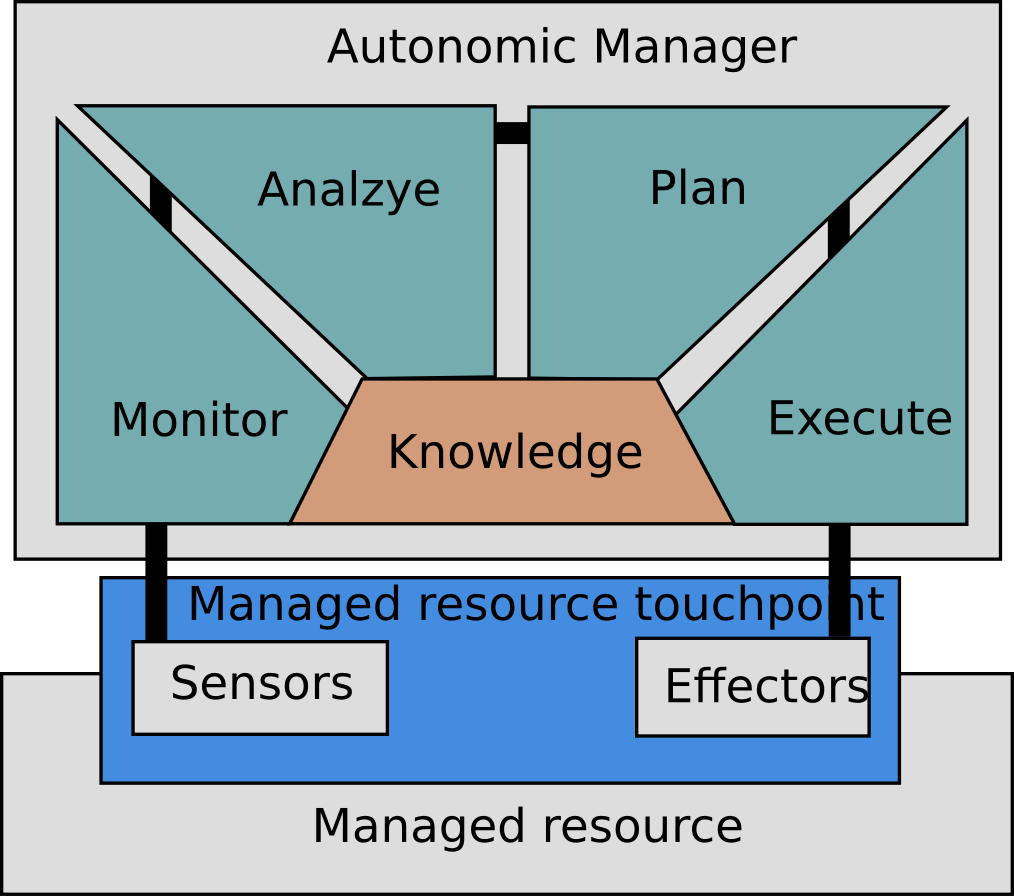
\includegraphics{01_introduccion/images/bucle-mape-k.png}
  \caption[Representación del Bucle MAPE-K]{Representación del Bucle MAPE-K.\footnotemark}
  \label{fig:bucle-mapek}
\end{figure}

% TODO: Cambiar por otra imagen sin typos.
\footnotetext{Obtenido de: \url{https://wwwvs.cs.hs-rm.de/vs-wiki/index.php/(WS12-01)_Cloud/Dokumentation}}


El recurso manejado puede ser un sistema \emph{hardware} o \emph{software} cualquiera. El único requisito es que debe implementar los \textbf{\emph{touchpoints}} (\textcolor{red}{puntos de contacto?}): interfaces que permiten al bucle de control obtener información del estado del sistema y cambiar su configuración en base a las políticas. Hay dos tipos de \emph{touchpoints}: \textbf{sondas} y \textbf{efectores}.

Las sondas reportan al bucle información del estado del sistema. Puede ser cualquier tipo de métrica que queramos controlar. Por ejemplo, \emph{health checks}, información de salud de la aplicación; propiedades del sistema que queramos controlar.

Por otro lado, los efectores, nos ayudan a modificar el estado del sistema manejado. Pueden ser ficheros de configuración, comandos, etc.

En la figura \ref{fig:bucle-mapek} podemos apreciar que el bucle puede dividirse en 5 componentes distintos: \cite{ArchitecturalBlueprintAutonomic2006}

\begin{itemize}
  \item \textbf{Base de conocimiento}: almacena el conocimiento relevante para la operación del bucle de control. Es tanto información del sistema como información del entorno de operación. Cada una de las claves almacenadas se conoce también como \textbf{propiedad de adaptación}.

  El conocimiento se comparte entre todos los componentes del bucle de control.

  \item \textbf{Monitor}: Recibe mediciones de las sondas del recurso manejado. Se encarga de recoger, agregar y filtrar estas mediciones para determinar si ha ocurrido un evento relevante que deba ser reportado. Por ejemplo, si la temperatura de una habitación supera un umbral definido por el usuario.

  \item \textbf{Analizador}: Conjunto de \textbf{reglas de adaptación} que se suscriben a las propiedades de adaptación. Están compuestas una condición y una acción. Cada vez que cambie alguna de las propiedades de las que dependen, se evalua su condición. Si esta se cumple, se ejecuta la acción asociada, que suele ser una propuesta de cambio en la configuración del sistema.

  \item \textbf{Planificador}: Si se ha llegado a ejecutar alguna regla de apdatación, el planificador recoge sus propuestas de cambio y determina las acciones necesarias para cumplir el objetivo.

  \item \textbf{Ejecutor}: Recibe
\end{itemize}


En este trabajo se quiere abordar la división de un servicio monolítico y adaptarlo para su funcionamiento en entornos en la nube. Para ello, se quiere extraer su funcionalidad en distintos microservicios. Es decir, se quiere \textbf{cambiar la topología} de la solución. Se trata de un cambio importante en la arquitectura de la solución.

%% TODO: ¿Multi-tennant? ¿Solución inicial muy acoplada y ad-hoc a una solución concreta? Se quiere independizar del programa.

La idea es separar cada una de sus etapas en microservicios individuales. De esta forma, podemos desarrollarlas de forma independiente entre ellas, replicarlas para mejorar su escalabilidad, o sustituirlas por implementaciones distintas, etc.

Para desarrollar el trabajo, propusimos el siguiente plan:
\begin{itemize}
  \item Cada etapa del bucle será un microservicio distinto. Extraeremos cuatro microservicios distintos: Planificador, Analizador,
\end{itemize}

Por tanto, los conectores elegidos para comunicar los microservicios han sido más centrados en comunicar con las APIs públicas que expone cada uno.

\section{Motivación}

????? ????????????? ????????????? ????????????? ????????????? ?????????????

\section{Objetivos}

????? ????????????? ????????????? ????????????? ????????????? ?????????????

\section{Estructura de la memoria}

????? ????????????? ????????????? ????????????? ????????????? ?????????????

%\section{Notes bibliografiques} %%%%% Opcional

%????? ????????????? ????????????? ????????????? ????????????? ?????????????
